\documentclass{report}
\usepackage{amsmath}
\usepackage{hyphenat}
\usepackage[shortlabels]{enumitem}
\usepackage{tikz}
\usepackage{fancyhdr}

\title{CS-23-01 Assignment 0}
\author{CJ Bridgman-Ford}
\date{February 12, 2024}

\newcommand{\pagenumber}{\thepage\quad}
\newcommand{\authorname}{CJ Bridgman-Ford}

\begin{document}

\pagestyle{fancy}
\renewcommand{\headrulewidth}{0pt}
\fancyfoot[L]{\authorname}
\fancyfoot[C]{}
\fancyfoot[R]{\pagenumber}


\maketitle



\begin{center}
\parbox{11.325cm}{
\begin{flushleft}
{Say we had a "black box," which takes two numbers as input and outputs their sum. See Figure 1.7a. Say we had another box capable of multiplying two numbers together. See figure 1.7b. We can connect these boxes together to calculate \(p \times (m + n )\). See Figure 1.7c. Assume we have an unlimited number of these boxes. Show how to connect them together to calculate:}
\end{flushleft}
\begin{enumerate}[(a)]
    \item{\(ax+b\)}
    \item{The average of the four input numbers \(w\), \(x\), \(y\), and \(z\)}
    \item{\(a^2+2ab+b^2\) (Can you do it with one add box and one multiply box?)}
\end{enumerate}
}

\vspace{5cm}

\parbox{11.325cm}{
\begin{flushleft}
{The discussion of abstraction in Section 1.3.1 noted that one does not need to understand the makeup of the components as long as "everything about the detail is just fine." The case was made that when everything is not fine, one must be able to deconstruct the components, or be at the mercy of the abstractions. In the taxi example, supposed you did not understand the component, that is, you had no clue how to get to the airport. Using the notion of abstraction, you simply tell the driver,}
\end{flushleft}
}

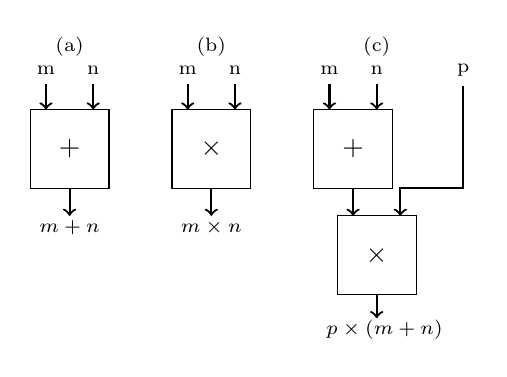
\begin{tikzpicture}
\node (a) at (0,1.3) {\scriptsize (a)};
\node (b) at (1.8,1.3) {\scriptsize (b)};
\node (c) at (3.9,1.3) {\scriptsize (c)};
\node (m1) at (-0.3,1) {\scriptsize m};
\node (n1) at (0.3,1) {\scriptsize n};
\node (m2) at (1.5,1) {\scriptsize m};
\node (n2) at (2.1,1) {\scriptsize n};
\node (m3) at (3.3,1) {\scriptsize m};
\node (n3) at (3.9,1) {\scriptsize n};
\node (p1) at (5,1) {\scriptsize p};
\node (b1) [draw, rectangle, minimum size=1cm] at (0,0) {+};
\node (b2) [draw, rectangle, minimum size=1cm] at (1.8,0) {\(\times\)};
\node (b3) [draw, rectangle, minimum size=1cm] at (3.6,0) {+};
\node (b4) [draw, rectangle, minimum size=1cm] at (3.9,-1.35) {\(\times\)};
\node (e1) at (0,-1) {\scriptsize \(m + n\)};
\node (e2) at (1.8,-1) {\scriptsize \(m \times n\)};
\node (e3) at (4,-2.3) {\scriptsize \(p \times (m+n)\)};

\draw[->, thick] (m1.south) -- (-0.3,0.5);
\draw[->, thick] (n1.south) -- (0.3,0.5);
\draw[->, thick] (m2.south) -- (1.5,0.5);
\draw[->, thick] (n2.south) -- (2.1,0.5);
\draw[->, thick] (m3.south) -- (3.3,0.5);
\draw[->, thick] (n3.south) -- (3.9,0.5);
\draw[->, thick] (p1.south) -- (5,-0.5) -- (4.2,-0.5) -- (4.2,-0.85);
\draw[->, thick] (b1.south) -- (0,-0.85);
\draw[->, thick] (b2.south) -- (1.8,-0.85);
\draw[->, thick] (b3.south) -- (3.6,-0.85);
\draw[->, thick] (b4.south) -- (3.9,-2.15);

\end{tikzpicture}

\newpage

\parbox{11.7cm}{
\begin{flushleft}
{Are items \(a\) through \(e\) in the following list algorithms? If not, what qualities required of algorithms do they lack?}

\begin{enumerate}[(a)]
    \item{Add the first row of the following matrix to another row whose first column contains a nonzero entry. (\textit{Reminder}: Columns run vertically; rows run horizontally.)}
\end{enumerate}
\end{flushleft}
}

$
\begin{bmatrix}
    1 & 2 & 0 & 4 \\
    0 & 3 & 2 & 4 \\
    2 & 3 & 10 & 22 \\
    12 & 4 & 3 & 4 
\end{bmatrix}
$

\vspace{5cm}

\parbox{11.5cm}{
\begin{flushleft}
{Fill in the following truth table for a one-bit AND operation.}    
\end{flushleft}
}
\begin{tabular}{c c|c}
\hline
X & Y & X AND Y \\
\hline
0 & 0 & \\
0 & 1 & \\
1 & 0 & \\
1 & 1 & \\
\hline
\end{tabular}

\end{center}
\end{document}
